\documentclass{beamer-control}
\usepackage{beamer-control-singlefile}
\INCLUDEONLY{Robust Pole Placement}
\begin{document}
\CONCEPT{Robust Pole Placement}

\begin{SUMMARY}
\begin{itemize}
\item Pole placement sensitivity
\item Design rules
\end{itemize}
\vfill References:
\begin{itemize}
\item \astrom{§14.5}
\end{itemize}
\end{SUMMARY}



\SUBCONCEPT{Pole placement sensitivity}

\begin{frame}{Robustness to process variation}
\begin{itemize}
\item We have seen that if a system is reachable we may assign the eigenvalues of the closed loop system, a technique known as pole placement
\item Care must be taken to make design choices that are robust to uncertainties in the system
\item Let us look at a couple of examples where we make reasonable designs but get poor performance
\end{itemize}
\end{frame}


\begin{frame}{Fast stable process poles}
\begin{itemize}
\item A pole is stable if it is in the left half-plane and unstable if it is in the right half-plane
\item A \textit{fast} pole is one that has a magnitude larger than the intended closed loop bandwidth
\item Consider a PI controller for a first-order system
\[P(s) = \frac{b}{s+a}, \quad C(s)=k_p+\frac{k_i}{s}\]
\item The closed loop characteristic polynomial is 
\[s(s+a)+b(k_ps+k_i)=s^2+(a+bk_p)s+k_ib\]
\item If we want poles at $-p_1$ and $-p_2$ we get
\[k_p=\frac{p_1+p_2-a}{b}, \quad k_i=\frac{p_1p_2}{b}\]
\end{itemize}
\end{frame}


\begin{frame}{Fast stable process poles}
	\begin{itemize}
		\item The sensitivity functions are 
		\[S(s) = \frac{s(s+a)}{(s+p_1)(s+p_2)}, \quad T(s) = \frac{(p_1+p_2-a)s+p_1p_2}{(s+p_1)(s+p_2)}\]
		\item Assume that pole $a$ is faster than the closed loop poles, the proportional gain $k_p$ is then negative and the controller has a zero in the right half-plane
		\item There is a large sensitivity peak due to the fast stable pole $\rightarrow$ poor robustness
	\end{itemize}
\begin{figure}
	\vspace{-0.5cm}
	\centering
	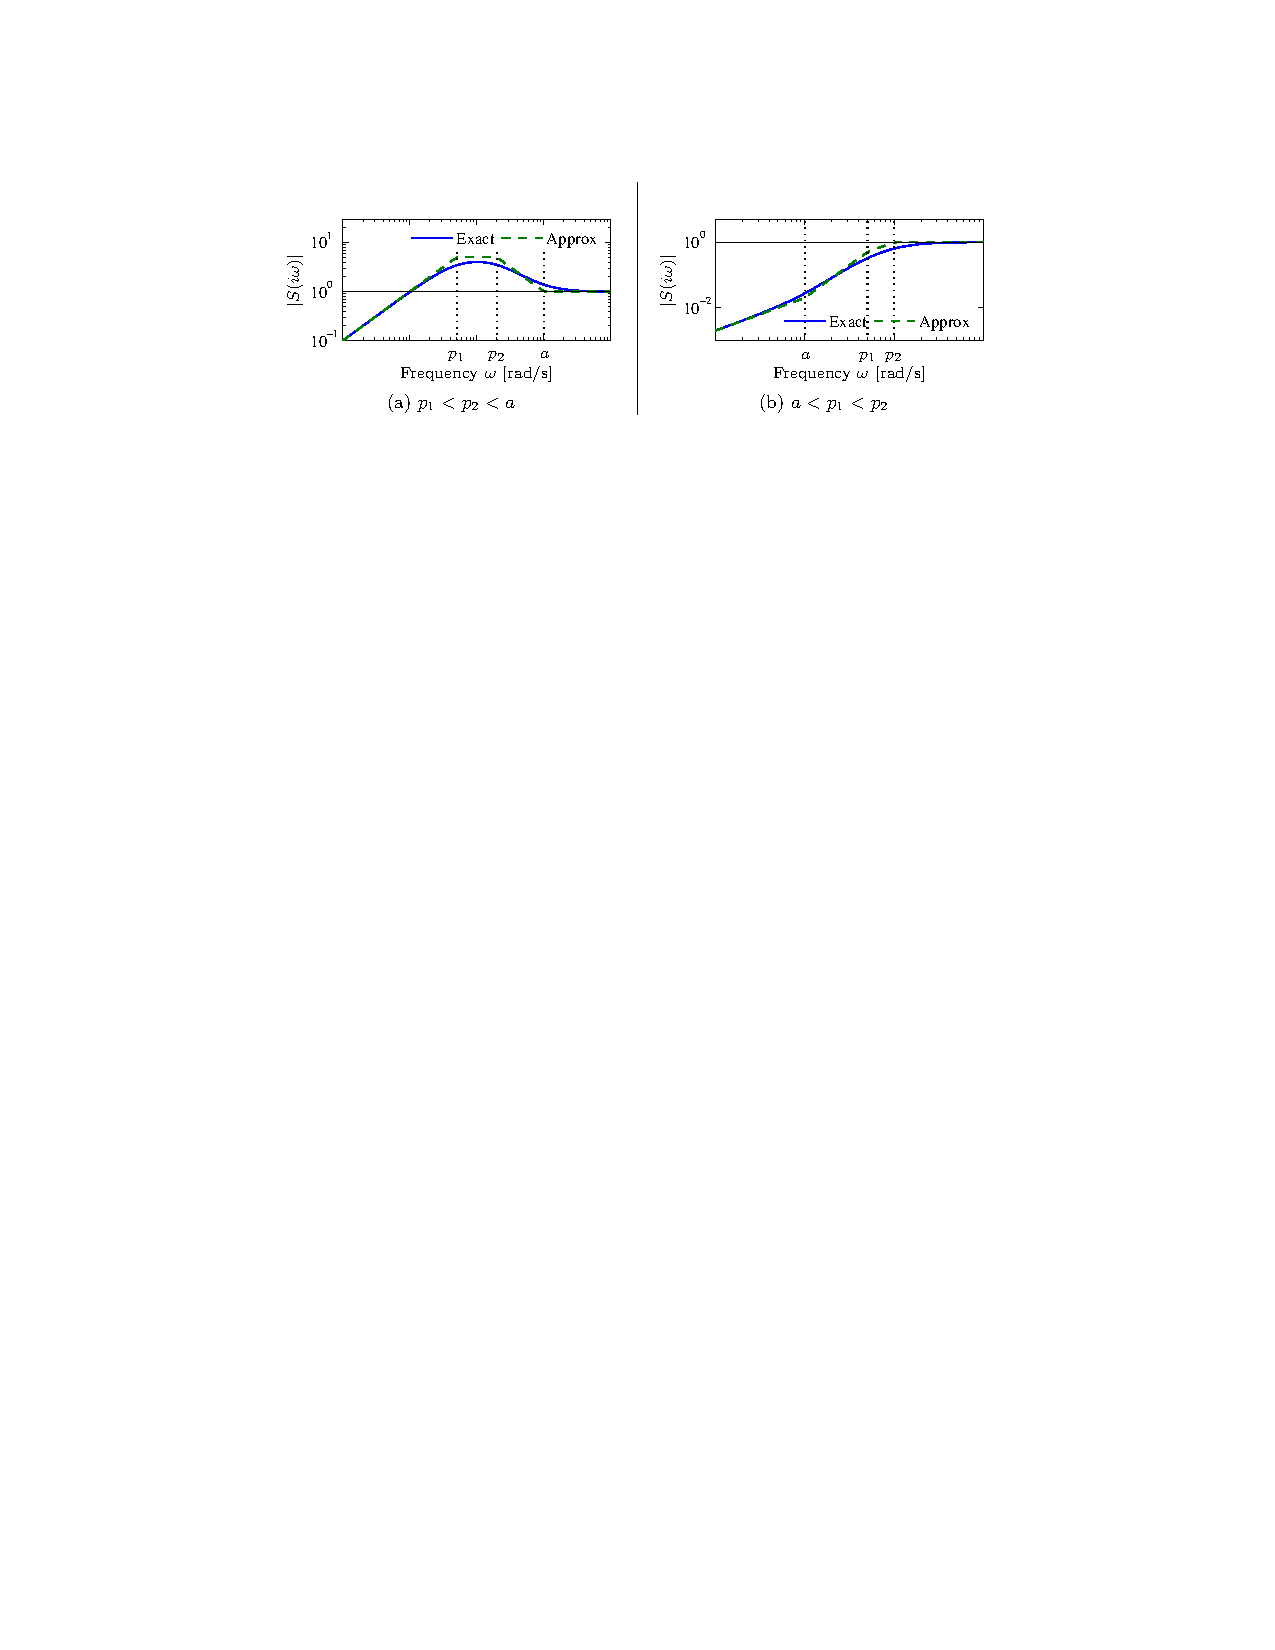
\includegraphics[width=10cm]{figure14.9}\\
	\vspace{-0.2cm}
	\textbf{Figure 14.9:} Gain curves of the sensitivity function.
\end{figure}
\end{frame}


\begin{frame}{Slow stable process zeros}
	\begin{itemize}
		\item A zero is \textit{slow} if its magnitude is smaller than the intended closed loop bandwidth
		\item Consider the vehicle steering system where the transfer function from steering angle to lateral position is 
		\[P(s)=\gamma \frac{s+1/\gamma}{s^2}\]
		\item This system has a slow stable zero at $s=-1/\gamma$
		\item A controller based on state feedback with an observer (Example 8.4) gives a controller 
		\[C(s) = \frac{-11516s+40000}{s^2+42.4s+6657.9}\]
	\end{itemize}
\end{frame}


\begin{frame}{Slow stable process zeros}
	\begin{itemize}
		\item Plotting the sensitivity functions shows a large peak 
		\item This peak can be avoided by assigning a closed loop pole at the slow process zero (or near it)
		\item This controller pole cancels the process zero and shows improved robustness
	\end{itemize}
	\begin{figure}
		\centering
		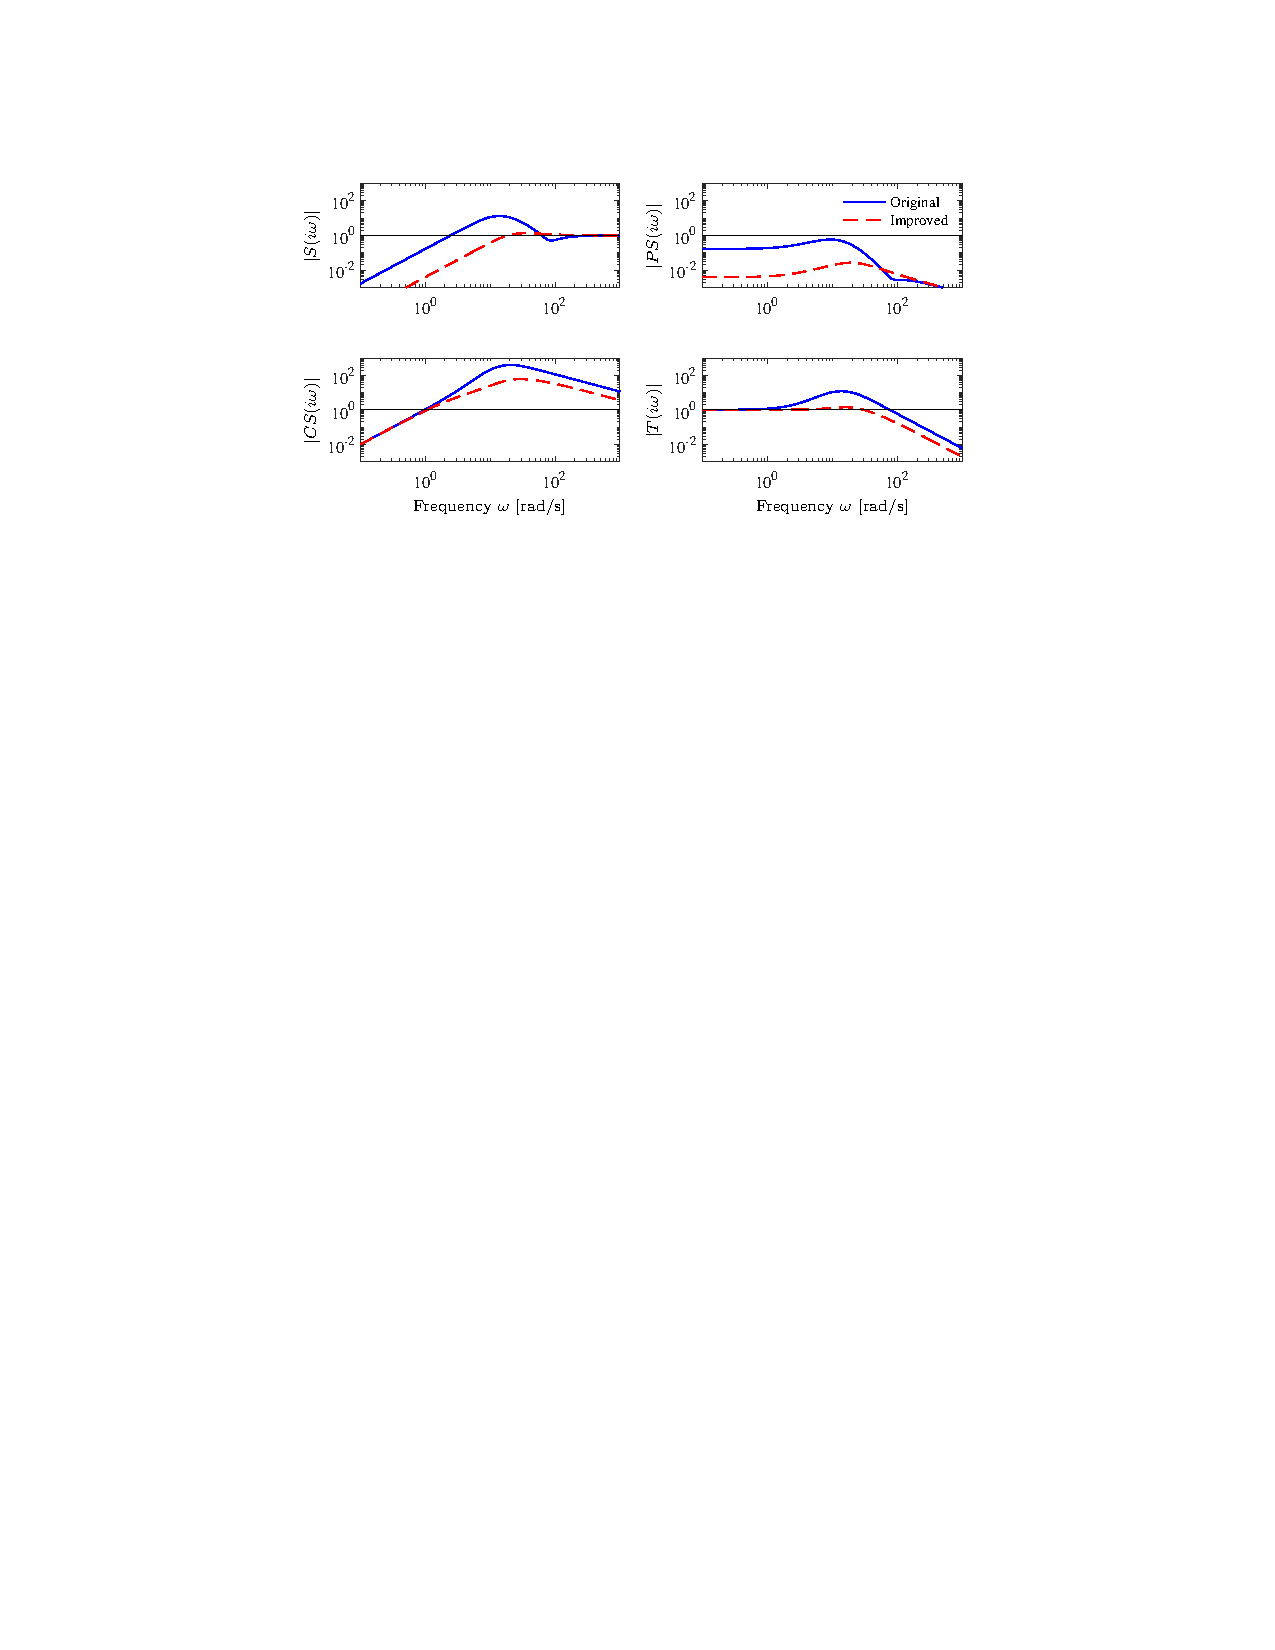
\includegraphics[width=9cm]{figure14.11}\\
		\vspace{-0.2cm}
		\textbf{Figure 14.11:} Gain curves of the sensitivity functions.
	\end{figure}
\end{frame}



\SUBCONCEPT{Design rules}

\begin{frame}{Good, robust pole placement}
	\begin{itemize}
		\item These examples give us some important insight in designing robust pole placement methods
		\item Slow stable zeros should be cancelled by controller poles to avoid peaks in the complementary sensitivity
		\item The peaks in sensitivity of fast stable poles should be minimised by having controller zeros close to the fast poles
		\item Slow unstable process zeros and fast unstable proces poles impose severe limits on the closed loop performance 
	\end{itemize}
\end{frame}

\SUMMARYFRAME
\FINALE

\end{document}
